\documentclass[12pt,a4paper,titlepage,twoside,openright]{article}
\usepackage{ucs} 
\usepackage[utf8x]{inputenc}
\usepackage[usenames,dvipsnames]{xcolor}
\usepackage{tikz}
\usepackage{caption}
\usepackage{latexsym}
\usepackage{amssymb}
\usepackage{amsmath}
\usepackage{subcaption} 

\usetikzlibrary{arrows} 
\usetikzlibrary{positioning} 
\usetikzlibrary{shapes} 
\usetikzlibrary{fit} 
\usetikzlibrary{backgrounds} 
\usetikzlibrary{calc}

\begin{document}
\begin{figure}
    \begin{subfigure}[b]{0.27\textwidth}
        \centering
        \resizebox{\linewidth}{!}{
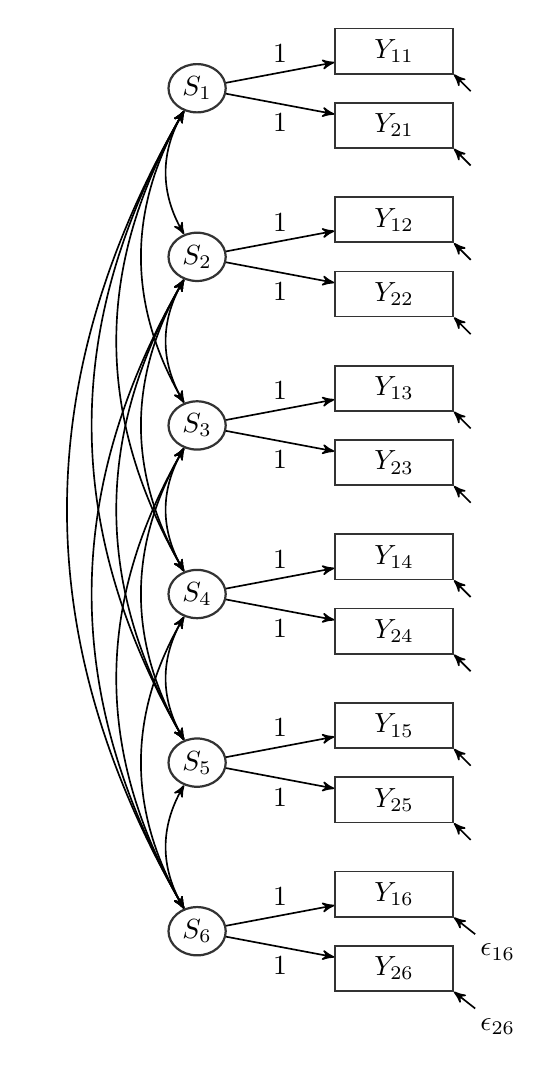
\begin{tikzpicture}
        [manifest/.style={rectangle,draw=black!80,semithick,minimum width=1.5cm,inner sep=
4pt,text centered},
        latent/.style={ellipse,draw=black!80,thick,inner sep=2,text centered},
        on/.style={->,>=stealth',semithick},
        from/.style={<-,>=stealth',semithick},
        with1/.style={<->,>=stealth',semithick,bend left=30},
        with2/.style={<->,>=stealth',semithick,bend right=30},
        with3/.style={<->,>=stealth',semithick,bend left=50},]

% Latent Variables %
 \begin{scope}[node distance=1.5]
                \node[latent] (o1) at (0,0) {$S_{1}$};
                \node[latent] (o2) [below=of o1] {$S_{2}$};
                \node[latent] (o3) [below=of o2] {$S_{3}$};
                \node[latent] (o4) [below=of o3] {$S_{4}$};
                \node[latent] (o5) [below=of o4] {$S_{5}$};
                \node[latent] (o6) [below=of o5] {$S_{6}$};
\end{scope}
                                                             	                        
% Manifest % 
 \foreach \a in {1,...,6} {\node (y1\a) [right = 2 of o\a] (yhelp\a) {};}        
 \foreach \b in {1,...,6} {\node[manifest] [above = .05 of yhelp\b] (y1\b) {$Y_{1\b}$}
 	edge [from] node[above] {1} (o\b);}
 \foreach \c in {1,...,6} {\node[manifest] [below = .05 of yhelp\c] (y2\c) {$Y_{2\c}$}
 	edge [from] node[below] {$1$} (o\c);} 

% Fehler %
\foreach \a in {1,...,5} {\node (e1\a) [below right = .3 of y1\a] {}
	edge [on] (y1\a.south east);}
\foreach \b in {1,...,5} {\node (e2\b) [below right = .3 of y2\b] {}
	edge [on] (y2\b.south east);}

\node (e16) [below right = .3 of y16] {$\epsilon_{16}$}
	edge [on] (y16.south east);
\node (e26) [below right = .3 of y26] {$\epsilon_{26}$}
	edge [on] (y26.south east);

%correlations%
\foreach \a in {1,...,5} {
\draw[<->,>=stealth',semithick] (o\a) to [with2]
node[align=center,below,yshift= 0mm, pos=0.5] 
                      {}  (o6);}
\foreach \a in {1,...,4} {
\draw[<->,>=stealth',semithick] (o\a) to [with2]
node[align=center,below,yshift= 0mm, pos=0.5] 
                      {}  (o5);}
\foreach \a in {1,...,3} {
\draw[<->,>=stealth',semithick] (o\a) to [with2]
node[align=center,below,yshift= 0mm, pos=0.5] 
                      {}  (o4);}
\foreach \a in {1,...,2} {
\draw[<->,>=stealth',semithick] (o\a) to [with2]
node[align=center,below,yshift= 0mm, pos=0.5] 
                      {}  (o3);}      
\draw[<->,>=stealth',semithick] (o1) to [with2]
node[align=center,below,yshift= 0mm, pos=0.5] 
                      {}  (o2);                

\end{tikzpicture}
        }
        \caption{Subfigure A}
    \end{subfigure}
    \begin{subfigure}[b]{0.34\textwidth}
    \centering
        \resizebox{\linewidth}{!}{
            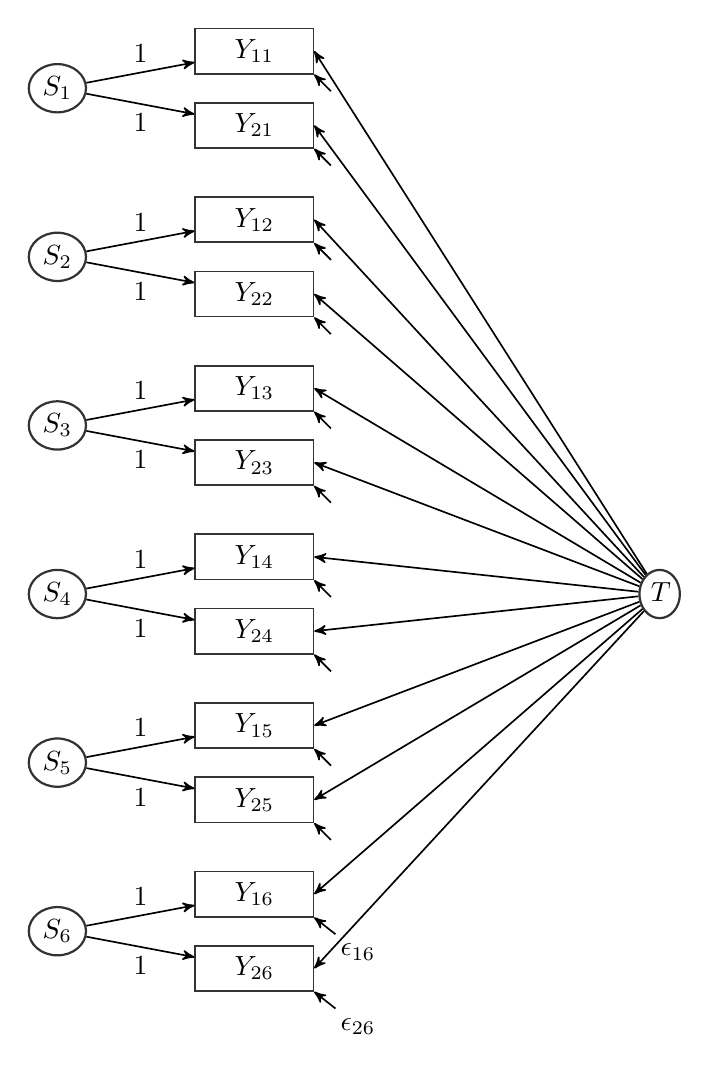
\begin{tikzpicture}
        [manifest/.style={rectangle,draw=black!80,semithick,minimum width=1.5cm,inner sep=
4pt,text centered},
        latent/.style={ellipse,draw=black!80,thick,inner sep=2,text centered},
        on/.style={->,>=stealth',semithick},
        from/.style={<-,>=stealth',semithick},
        with1/.style={<->,>=stealth',semithick,bend left=30},
        with2/.style={<->,>=stealth',semithick,bend right=30},
        with3/.style={<->,>=stealth',semithick,bend left=50},]
        
% Latent Variables %
 \begin{scope}[node distance=1.5]
                \node[latent] (o1) at (0,0) {$S_{1}$};
                \node[latent] (o2) [below=of o1] {$S_{2}$};
                \node[latent] (o3) [below=of o2] {$S_{3}$};
                \node[latent] (o4) [below=of o3] {$S_{4}$};
                \node[latent] (o5) [below=of o4] {$S_{5}$};
                \node[latent] (o6) [below=of o5] {$S_{6}$};
\end{scope}
                     
% Trait % 
\node[latent,node distance=7] (t) [right=of  o4]  {$T_{}$};
                                             	                        
% Manifest % 
 \foreach \a in {1,...,6} {\node (y1\a) [right = 2 of o\a] (yhelp\a) {};}        
 \foreach \b in {1,...,6} {\node[manifest] [above = .05 of yhelp\b] (y1\b) {$Y_{1\b}$}
 	edge [from] node[above] {1} (o\b);}
 \foreach \c in {1,...,6} {\node[manifest] [below = .05 of yhelp\c] (y2\c) {$Y_{2\c}$}
 	edge [from] node[below] {$1$} (o\c);} 

% Fehler %
\foreach \a in {1,...,5} {\node (e1\a) [below right = .3 of y1\a] {}
	edge [on] (y1\a.south east);}
\foreach \b in {1,...,5} {\node (e2\b) [below right = .3 of y2\b] {}
	edge [on] (y2\b.south east);}

\node (e16) [below right = .3 of y16] {$\epsilon_{16}$}
	edge [on] (y16.south east);
\node (e26) [below right = .3 of y26] {$\epsilon_{26}$}
	edge [on] (y26.south east);

% Pfeile %
\foreach \a in {1,...,6}
	\path (y1\a.0) edge [from] (t);
\foreach \a in {1,...,6}	
	\path (y2\a.0) edge [from] (t);
\end{tikzpicture}
        }
        \caption{Subfigure B}   
    \end{subfigure}
    \begin{subfigure}[b]{0.37\textwidth}
        \centering
        \resizebox{\linewidth}{!}{
  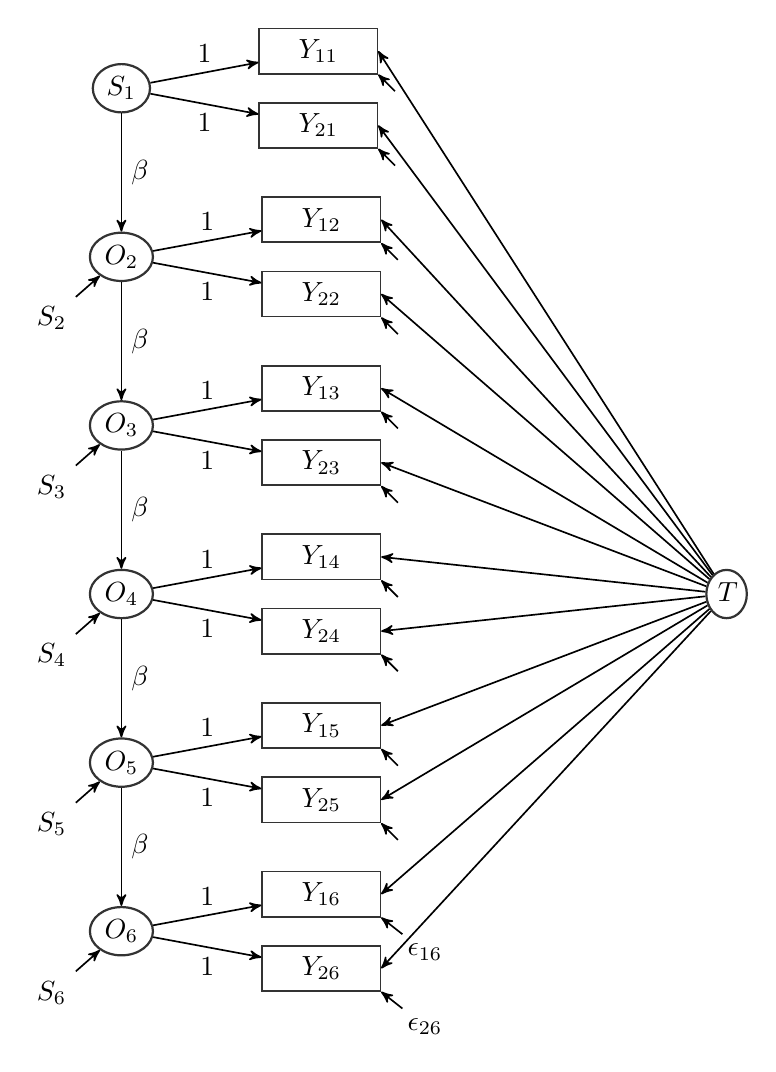
\begin{tikzpicture}
 [manifest/.style={rectangle,draw=black!80,semithick,minimum width=1.5cm,inner sep=
4pt,text centered},
        latent/.style={ellipse,draw=black!80,thick,inner sep=2,text centered},
        on/.style={->,>=stealth',semithick},
        from/.style={<-,>=stealth',semithick},
        with1/.style={<->,>=stealth',semithick,bend left=30},
        with2/.style={<->,>=stealth',semithick,bend right=30},
        with3/.style={<->,>=stealth',semithick,bend left=50},]


% Latent Variables %
 \begin{scope}[node distance=1.5]
                \node[latent] (o1) at (0,0) {$S_{1}$};
                \node[latent] (o2) [below=of o1] {$O_{2}$}
                edge [from] node[right] {$\beta$} (o1);
                \node[latent] (o3) [below=of o2] {$O_{3}$}
                edge [from] node[right] {$\beta$} (o2);
                \node[latent] (o4) [below=of o3] {$O_{4}$}
                edge [from] node[right] {$\beta$} (o3);
                \node[latent] (o5) [below=of o4] {$O_{5}$}
                edge [from] node[right] {$\beta$} (o4);
                \node[latent] (o6) [below=of o5] {$O_{6}$}
                edge [from] node[right] {$\beta$} (o5);
\end{scope}

\foreach \a in {2,...,6} {\node [below left = .4 of o\a] (zeta\a) {$S_{\a}$}
	edge [on] (o\a);}
                     
% Trait % 
\node[latent,node distance=7] (t) [right=of  o4]  {$T_{}$};
                                             	                        
% Manifest % 
 \foreach \a in {1,...,6} {\node (y1\a) [right = 2 of o\a] (yhelp\a) {};}        
 \foreach \b in {1,...,6} {\node[manifest] [above = .05 of yhelp\b] (y1\b) {$Y_{1\b}$}
 	edge [from] node[above] {1} (o\b);}
 \foreach \c in {1,...,6} {\node[manifest] [below = .05 of yhelp\c] (y2\c) {$Y_{2\c}$}
 	edge [from] node[below] {$1$} (o\c);} 

% Fehler %
\foreach \a in {1,...,5} {\node (e1\a) [below right = .3 of y1\a] {}
	edge [on] (y1\a.south east);}
\foreach \b in {1,...,5} {\node (e2\b) [below right = .3 of y2\b] {}
	edge [on] (y2\b.south east);}

\node (e16) [below right = .3 of y16] {$\epsilon_{16}$}
	edge [on] (y16.south east);
\node (e26) [below right = .3 of y26] {$\epsilon_{26}$}
	edge [on] (y26.south east);

% Pfeile %
\foreach \a in {1,...,6}
	\path (y1\a.0) edge [from] (t);
\foreach \a in {1,...,6}	
	\path (y2\a.0) edge [from] (t);
\end{tikzpicture}
        }
        \caption{Subfigure C}
    \end{subfigure}
\end{figure}

\end{document}